%%%%%%%%%%%%%%%%%%%%%%%%%%%%%%%%%%%%%%%%%
% The Legrand Orange Book
% LaTeX Template
% Version 2.1.1 (14/2/16)
%
% This template has been downloaded from:
% http://www.LaTeXTemplates.com
%
% Original author:
% Mathias Legrand (legrand.mathias@gmail.com) with modifications by:
% Vel (vel@latextemplates.com)
%
% License:
% CC BY-NC-SA 3.0 (http://creativecommons.org/licenses/by-nc-sa/3.0/)
%
% Compiling this template:
% This template uses biber for its bibliography and makeindex for its index.
% When you first open the template, compile it from the command line with the 
% commands below to make sure your LaTeX distribution is configured correctly:
%
% 1) pdflatex main
% 2) makeindex main.idx -s StyleInd.ist
% 3) biber main
% 4) pdflatex main x 2
%
% After this, when you wish to update the bibliography/index use the appropriate
% command above and make sure to compile with pdflatex several times 
% afterwards to propagate your changes to the document.
%
% This template also uses a number of packages which may need to be
% updated to the newest versions for the template to compile. It is strongly
% recommended you update your LaTeX distribution if you have any
% compilation errors.
%
% Important note:
% Chapter heading images should have a 2:1 width:height ratio,
% e.g. 920px width and 460px height.
%
%%%%%%%%%%%%%%%%%%%%%%%%%%%%%%%%%%%%%%%%%

%----------------------------------------------------------------------------------------
%	PACKAGES AND OTHER DOCUMENT CONFIGURATIONS
%----------------------------------------------------------------------------------------

\documentclass[11pt,fleqn]{book} % Default font size and left-justified equations

\usepackage{wasysym}
\usepackage{esint} % various fancy integral symbols
\usepackage{tikz}
\usepackage{tikz-3dplot}
\usepackage{pgfplots}
\pgfplotsset{compat=1.17}
\usetikzlibrary{patterns}
\usepackage{tkz-euclide} 
\usepackage{mathtools}
\usepackage{xurl}
\usepackage[version=4,arrows=pgf-filled,
textfontname=sffamily,
mathfontname=mathsf]{mhchem}
\usepackage{gensymb}
\usepackage[french]{babel}

\usetikzlibrary {arrows.meta} 

\newcommand{\degC}{{\degree}C}
\newcommand{\dd}{\mathrm{d}}
\newcommand{\div}{\mathrm{div}}
\newcommand{\rot}{\vv{\mathrm{div}}}
\newcommand{\grad}{\vv{\mathrm{grad}}}

\tikzset{
    support/.style={
        pattern=north east lines,
        draw=none,
        minimum width=0.3,
        minimum height=0.6
    }
    ,>=latex
}

\usepackage[d]{esvect}

%SPECIFIC TO THIS CHAPTER
\usepackage{physics}
\usepackage{ifthen}
\usepackage[outline]{contour} % glow around text
\usetikzlibrary{calc} % for pic
\usetikzlibrary{angles,quotes} % for pic
\usetikzlibrary{patterns}
\tikzset{>=latex} % for LaTeX arrow head
\contourlength{1.2pt}

\colorlet{myred}{red!65!black}
\definecolor{myred}{RGB}{255,81,46}
\tikzstyle{ground}=[preaction={fill,top color=black!10,bottom color=black!5,shading angle=20},
                    fill,pattern=north east lines,draw=none,minimum width=0.3,minimum height=0.6]
\tikzstyle{mass}=[line width=0.6,myred,fill=myred!40,rounded corners=1,
                  top color=myred!40,bottom color=myred!20,shading angle=20]
\tikzstyle{rope}=[myred!30,line width=1.2,line cap=round] %very thick

% FORCES SWITCH
\tikzstyle{force}=[->,myred,ultra thick,line cap=round]
\tikzstyle{Fproj}=[force,myred!60]
\newboolean{showforces}
\setboolean{showforces}{true}
%----------------------------------------------------------------------------------------

\input{structure} % Insert the commands.tex file which contains the majority of the structure behind the template

\begin{document}

%----------------------------------------------------------------------------------------
%	TABLE OF CONTENTS
%----------------------------------------------------------------------------------------

%\usechapterimagefalse % If you don't want to include a chapter image, use this to toggle images off - it can be enabled later with \usechapterimagetrue

\chapterimage{gas_stove_flame.jpg} % Table of contents heading image

%\pagestyle{empty} % No headers

%\tableofcontents % Print the table of contents itself

%\cleardoublepage % Forces the first chapter to start on an odd page so it's on the right

%\pagestyle{fancy} % Print headers again



%\part{\'{E}lectromagnétisme}

\setcounter{chapter}{4}

\chapter{\'{E}nergie chimique}

Dans ce chapitre et le suivant, nous allons nous intéresser à la thermodynamique chimique, aussi appelée thermochimie. La thermodynamique chimique s'intéresse aux transferts d'énergie et d'entropie dans les systèmes chimiques. Elle a de nombreuses applications dans la vie quotidienne et dans l'industrie. En particulier, dans ce chapitre, nous allons nous intéresser à l'énergie présente sous forme chimique (par exemple dans les combustibles comme l'essence). 

\section{Introduction : l'énergie chimique}

Nous pouvons commencer ce chapitre par l'analyse d'une réaction chimique : celle de la combustion. Lors d'une combustion, un combustible brûle et réagit avec un comburant. Le comburant est souvent sous forme gazeuse dans l'environnement, alors que le combustible peut être liquide, solide ou même gazeux. Un exemple caractéristique est la réaction de combustion du propane (\ce{C3H8}) que l'on utilise dans les cuisinières :
\begin{equation}
    \ce{C3H8 + 5 O2 -> 3 CO2 + 4 H2O}
\end{equation}
Ici, le propane réagit avec le dioxygène présent dans l'air pour former du dioxyde de carbone et de l'eau sous forme gazeuse (vapeur d'eau). Lorsque l'on effectue cette réaction, on constate un dégagement d'énergie thermique qui permet de chauffer les plats sur la cuisinière à 100 voire 200\degC. 

D'où vient cette énergie thermique ? Pour le comprendre, nous pouvons appliquer le premier principe de la thermodynamique. Considérons une cuisine dans laquelle se trouve une bonbonne de gaz reliée à une cuisinière sur laquelle se trouve une casserole. Nous choisissons d'étudier le système $\Sigma$ comprenant la bonbonne de gaz, la cuisinière, et l'air contenu dans la pièce. Pour simplifier notre raisonnement, on suppose que la casserole est déjà sur le feu depuis un certain temps, de sorte que la température du système $\Sigma$ est constante. En revanche, la casserole, elle, chauffe : elle reçoit une puissance thermique $\mathcal{P}$ de la part du système $\Sigma$.

Nous rappelons ici l'expression du premier principe :
\begin{theorem}[Premier principe de la thermodynamique (rappel)]
    Soit un système fermé $\Sigma$ subissant une transformation thermodynamique. Nous notons $\mathcal{U}$ son énergie interne, $\mathcal{E}_c$ son énergie cinétique macroscopique, et   $\mathcal{E}_p$ son énergie potentielle macroscopique. Nous notons également $Q$ l'énergie thermique reçue par le système au cours de la transformation, et $W$ le travail des forces extérieures sur le système pendant la transformation. Alors :
    \begin{equation}
        \Delta(\mathcal{U} + \mathcal{E}_p + \mathcal{E}_c) = W + Q
    \end{equation}
\end{theorem}


Le système $\Sigma$ est un système fermé, en effet le gaz qui sort de la bonbonne réagit avec le dioxygène mais les produits de combustion se mélangent à l'air de la pièce. On peut donc lui appliquer le premier principe. Le système $\Sigma$ n'a pas d'énergie cinétique macroscopique et son énergie potentielle est constante, par ailleurs les forces extérieures ne travaillent pas. Enfin l'énergie reçue par le système au cours d'une durée $\Delta t$ est donnée par $Q = -\mathcal{P} \Delta t$. On en déduit :
\begin{equation}
    \Delta \mathcal{U} = - \mathcal{P} \Delta t
\end{equation}
Cette équation nous montre que \textbf{l'énergie thermique libérée par la réaction chimique provient d'une variation d'énergie interne dans le système chimique}. Comment pouvons-nous expliquer ceci ?

Nous pouvons rappeler la définition de l'énergie interne vue en première année :
\begin{definition}[Énergie interne]
 L'énergie interne d'un système correspond à la somme de l'énergie potentielle et l'énergie cinétique contenues à l'échelle microscopique dans le système.
\end{definition}
Cette énergie est présente sous plusieurs formes :
\begin{itemize}
    \item Énergie cinétique des molécules 
    \item Énergie de liaison entre les molécules (liaisons de Van der Waals)
    \item Énergie de liaison à l'intérieur des molécules ou cristaux entre les atomes/ions
\end{itemize}
Dans notre cas, c'est de la troisième composante que provient l'énergie. Lors de la réaction de combustion, les liaisons C-H et C-C du propane et O=O du dioxygène sont cassées pour former des liaisons O-H et C=O qui sont énergétiquement plus favorables. De l'énergie électrostatique d'interaction entre les atomes est alors libérée et convertie en énergie thermique.

Dans le reste du chapitre, nous allons nous intéresser à ce processus de façon quantitative : comment prévoir combien d'énergie on peut retirer d'une réaction chimique ? Comment la température va varier au cours d'une réaction ?

\section{Enthalpie de réaction}

Pour quantifier ces transferts d'énergie, nous devons nous placer dans un cadre approprié. La définition du système auquel on a appliqué le premier principe dans le cas précédent n'était pas intuitive et surtout peu utile. En règle générale, les transformations chimiques ne se font pas à volume constant, surtout lorsque l'on a des gaz. En revanche, elles se font souvent à la pression atmosphérique, à laquelle le système s'ajuste très rapidement pendant ou juste après la réaction. Nous allons plutôt nous intéresser au cas d'une transformation au cours de laquelle la pression extérieure est constante. On parle d'une transformation monobare.

Nous rappelons quelques définitions :
\begin{definition}
    Une transformation est dite :
    \begin{itemize}
        \item \textbf{Monobare} si la pression extérieure est constante au cours de la transformation;
        \item \textbf{Isobare} si la pression est définie tout le long de la transformation (trasnformation quasi-statique) et que celle-ci est constante au cours de la transformation;
        \item \textbf{Monotherme} si la température extérieure est constante au cours de la transformation;
        \item \textbf{Isotherme} si la température est définie tout le long de la transformation (transformation quasi-statique) et que celle-ci est constante au cours de la transformation;
    \end{itemize}
\end{definition}

Nous avons vu en première année qua dans le cas d'une transformation isobare, il est utile de définir une nouvelle variable, appelée enthalpie :
\begin{definition}[Enthalpie (rappel)]
    L'enthalpie d'un système d'énergie interne $\mathcal{U}$, de volume $V$ et à la pression $p$ est donnée par :
    \begin{equation}
        \mathcal{H} = \mathcal{U} + p V
    \end{equation}
\end{definition}

Comme le système est à l'équilibre avec l'environnement au début et à la fin de la transformation, on peut remarquer que la pression dans le système est égale à la pression extérieure au début et à la fin de la transformation ($p_{finale} = p_{initiale} = p_{ext}$), si bien que :
\begin{equation}
    \Delta \mathcal{H} = \Delta \mathcal{U} + p_{finale} V_{final} - p_{initiale} V_{initial} = \Delta \mathcal{U} + p_{ext} \Delta V
\end{equation}

Le travail des forces extérieures lors d'une transformation monobare s'écrit :
\begin{equation}
    W = - \int p_{ext} \dd V = - p_{ext} \Delta V
\end{equation}
On obtient alors en appliquant le premier principe :
\begin{equation}
    \Delta (\mathcal{H} + \mathcal{E}_p + \mathcal{E}_c) = W_{autres} + Q
\end{equation}
où $W_{autres}$ correspond au travail des forces autres que les forces de pression. Dans le cas général d'une transformation chimique à l'air libre, la plupart de ces termes disparaissent :
\begin{proposition}
    Soit $\Sigma$ un système composé de réactifs chimiques. Lors d'une transformation chimique \textbf{monobare} entre deux états d'équilibre, si le système ne subit pas de variation d'énergie mécanique macroscopique et n'est pas soumis au travail de forces autres que les forces de pression, alors :
    \begin{equation}
        \Delta \mathcal{H} = Q
    \end{equation}
\end{proposition}

Cette relation est très utile pour décrire les réactions chimiques. En effet, elle relie directement les transferts thermiques lors de la réaction aux transferts thermiques entre le système et son environnement. Par ailleurs, la quantité $\Delta \mathcal{H}$ se décompose en deux parties :
\begin{itemize}
    \item Une contribution $\Delta \mathcal{H}_{chimique}$ issue de la rupture des liaisons des réactifs et de la formation de nouvelles liaisons. Il s'agit de la variation d'énergie potentielle microscopique du système ;
    \item Une contribution $\Delta \mathcal{H}_{thermique}$ issue de la variation de température du système. Il s'agit de la variation d'énergie cinétique microscopique du système correspondant à l'agitation thermique de ses consitutants.    
\end{itemize}

L'énergie chimique libérée par la réaction est donnée par la quantité $\Delta H_{chimique}$. Cette énergie est ensuite convertie en énergie thermique qui peut soit rester à l'intérieur du système et l'échauffer ou le refoidir ($\Delta \mathcal{H}_{thermique}$) ou bien être transférée à l'extérieur du système ($Q$). 

Ceci nous amène à définir la quantité $\Delta H_{chimique}$ de façon plus rigoureuse, puisqu'elle est la mesure de l'énergie pouvant être libérée par une réaction chimique. Il s'agit de la variation d'enthalpie du système chimique en l'absence de variation de pression ou de température. Pour définir cette quantité de manière claire, nous devons adopter certaines conventions.

\section{Enthalpie standard de réaction}

Nous commençons par définir l'état standard d'un composé chimique, dans lequel la pression est fixée à la pression atmosphérique $P \degree = P^\circ = 1$\,bar. Cet état va nous servir à tabuler les variations d'enthalpie lors d'une réaction chimique. Pour un corps pur, on choisit toujours comme état standard la phase de ce corps pur qui est stable à $P \degree = P^\circ$ et à la température spécifiée.

L'état standard des différentes phases ou états est défini comme suit :
\begin{definition}[Etat standard d'un gaz]
   Pour un composé gazeux, l'état standard est l'état de gaz parfait pur à la pression $P \degree$.
\end{definition}
\begin{definition}[Etat standard d'une phase condensée]
   Pour un composé solide ou liquide, y compris pour un solvant, l'état standard est l'état pur (non mélangé à une autre espèce) à la pression $P \degree$.
\end{definition}
\begin{definition}[Etat standard d'un soluté]
   Pour un composé en solution, l'état standard est l’état hypothétique de ce soluté dans le solvant lorsqu’il est infiniment dilué, à la pression $P \degree$ et à la concentration $C \degree = 1$\,mol$\cdot$L$^{-1}$. 
\end{definition}
\begin{remark}
    Cet état est évidemment hypothétique puisqu'on ne peut pas être infiniment dilué et à une concentration (relativement forte !) de 1\,mol$\cdot$L$^{-1}$. En pratique, cela signifie que l'on considère le soluté à la concentration de référence, mais on néglige les interactions entre les différentes molécules ou les différents ions du soluté (ce qui est le cas lorsque le soluté est infiniment dilué).
\end{remark}

Une fois que l'on a défini ces états standard, on peut définir de façon rigoureuse la variation d'enthalpie d'un système chimique lors d'une transformation. Pour cela, on suppose que tous les réactifs sont dans leur état standard avant la réaction, et tous les produits sont dans leur état standard après la réaction. On suppose que les réactifs sont en proportion stœchiométrique de sorte qu'il n'en reste aucun à la fin de la réaction. On définit ainsi l'enthalpie standard de réaction :
\begin{definition}[Enthalpie standard de réaction]
    L'enthalpie standard d'une réaction chimique est la variation d’enthalpie de la réaction théorique isotherme au cours de laquelle les réactifs en nombre de moles égaux aux coefficients stœchiométriques sont pris dans leur état standard, et se transforment entièrement en produits pris dans leur état standard. Elle se note $\Delta_r H \degree(T)$ et dépend de la température. Son unité est le kJ$\cdot$mol$^{-1}$.
    
    Mathématiquement :
    \begin{equation}
        \Delta_r H \degree(T) = \left.\frac{\partial H}{\partial \xi}\right|_{T,P}(T,P=P^\circ)
    \end{equation}
    où $\xi$ est l'avancement de la réaction.
\end{definition}

\begin{remark}
    Attention ! La façon dont on équilibre les coefficients stoechiométriques est importante. Si on multiplie par 2 les coefficients stoechiométriques, alors on multiplie aussi par 2 l'enthalpie standard. 
\end{remark}

Dans le cas d'une réaction à l'état standard et isotherme, on aura ainsi $\Delta \mathcal{H} = \Delta_r H \degree$. Or on a vu que $\Delta \mathcal{H} = Q$, autrement dit l'enthalpie de réaction correspond à l'énergie thermique reçue par le système au cours d'une transformation isotherme. Ceci nous fournit une interprétation concrète de l'enthalpie standard de réaction : 
\begin{proposition}
    L'enthalpie standard de réaction mesure, au signe près, l'énergie chimique (par unité d'avancement) pouvant être libérée sous forme thermique lors d'une réaction chimique.
\end{proposition}

On distingue alors deux cas de figure :
\begin{definition}
    Une réaction est dite exothermique si elle libère de l'énergie thermique ($Q<0$). Dans ce cas, l'enthalpie de réaction est négative.
\end{definition}
\begin{definition}
    Une réaction est dite endothermique si elle consomme de l'énergie thermique ($Q>0$). Dans ce cas, l'enthalpie de réaction est négative.
\end{definition}

\begin{example}
    Dans le cas d'une réaction de combustion comme la combustion du propane, l'enthalpie de réaction est négative. La réaction chimique fournit de l'énergie.
\end{example}

\subsection*{Exemple : température d'une flamme}

Nous allons appliquer le premier principe pour calculer la température d'une flamme. Considérons à nouveau la réaction de combustion du propane :
\begin{equation}
    \ce{C3H8 + 5 O2 -> 3 CO2 + 4 H2O}
\end{equation}
Nous considérons un système composé des réactifs gazeux à l'équilibre avant combustion, que nous supposons en quantité stœchiométrique et en l'absence d'autre gaz. 

Comme la transformation ne dépend pas du chemin suivi, on peut imaginer la transformation comme une succession de deux états :
\begin{itemize}
    \item Phase 1 : la réaction se produit à la température ambiante $T_0 \approx 300$\,K
    \item Phase 2 : les produits s'échauffent jusqu'à la température $T_f$ atteinte dans l'état final.
\end{itemize}

On peut alors écrire la variation d'enthalpie au cours de la réaction comme la somme de la variation d'enthalpie lors des deux étapes :
\begin{equation}
    \Delta \mathcal{H} = \Delta \mathcal{H}_1 + \Delta \mathcal{H}_2
\end{equation}

Commençons par calculer la variation d'enthalpie lors de la première phase.
L'enthalpie standard de la réaction est tabulée et vaut $\Delta_r H\degree = -2\,$MJ$\cdot$mol$^{-1}$. Comme les réactifs et produits forment un mélange de gaz, ils ne sont pas dans leur état standard. Cependant, nous avons vu en première année que pour un gaz parfait, l'enthalpie molaire ne dépend que de la température et pas de la pression partielle du gaz : $\mathcal{H} = c_p T$ (2e loi de Joule). Ainsi, en supposant que les réactifs et produits se comportent comme des gaz parfaits, l'enthalpie des réactifs gazeux réels est la même que leur enthalpie dans leur état standard. On en déduit que la variation d'enthalpie est la même que pour la réaction standard. Si une quantité de matière $n$ de propane est brûlée alors :
\begin{equation}
    \Delta \mathcal{H}_1 = n \Delta_r H\degree
\end{equation}

Dans la seconde phase, les produits sont échauffés. Ils correspondent à $3n$ moles de \ce{CO2} et $4n$ moles de \ce{H2O}. D'après la seconde loi de Joule, leur enthalpie ne dépend que de la température et comme il s'agit d'une grandeur extensive, on peut additionner l'enthalpie des deux gaz :
\begin{equation}
    H_2(T) = 3 n C_{p,\ce{CO2}} T + 4 n C_{p,\ce{H2O}} T
\end{equation}
d'où la variation d'enthalpie :
\begin{equation}
    \Delta \mathcal{H}_2 = (3 C_{p,\ce{CO2}} + 4 C_{p,\ce{H2O}}) n (T_f-T_0)
\end{equation}

Enfin, nous avons vu que si la réaction se produit en l'absence de changement d'énergie mécanique macroscopique et en l'absence de travaux de forces autres que les forces de pression :
\begin{equation}
    \Delta \mathcal{H} = Q
\end{equation}
La réaction étant supposée adiabatique, nous avons $Q = 0$. En remplaçant $\Delta \mathcal{H}$ par son expression nous obtenons :
\begin{equation}
    n \Delta_r H\degree + \Delta \mathcal{H}_2 = (3 C_{p,\ce{CO2}} + 4 C_{p,\ce{H2O}}) n (T_f-T_0) = 0
\end{equation}

Après avoir simplifié $n$ nous obtenons une estimation de la température finale :
\begin{equation}
    T_f = T_0 - \frac{\Delta_r H\degree}{3 C_{p,\ce{CO2}} + 4 C_{p,\ce{H2O}}}
\end{equation}
En utilisant les valeurs $C_{p,\ce{H2O}} = 36$\,J$\cdot$K$\cdot$mol$^{-1}$ et $C_{p,\ce{CO2}} = 37$\,J$\cdot$K$\cdot$mol$^{-1}$ on obtient une température de flamme :
\begin{equation}
    T_f \approx 8000\,\mathrm{K}
\end{equation}
Un corps porté à une telle température émet un rayonnement dont le spectre dépend de la température et est donnée par la loi de Wien (vue au lycée). La couleur résultant de ce spectre est indiquée sur la figure ci-dessus. On peut y constater qu'une température de 8000\,K correspond à une couleur bleutée, qui est effectivement la couleur de la flamme sortant d'une cuisinière.

\begin{figure}
    \centering
    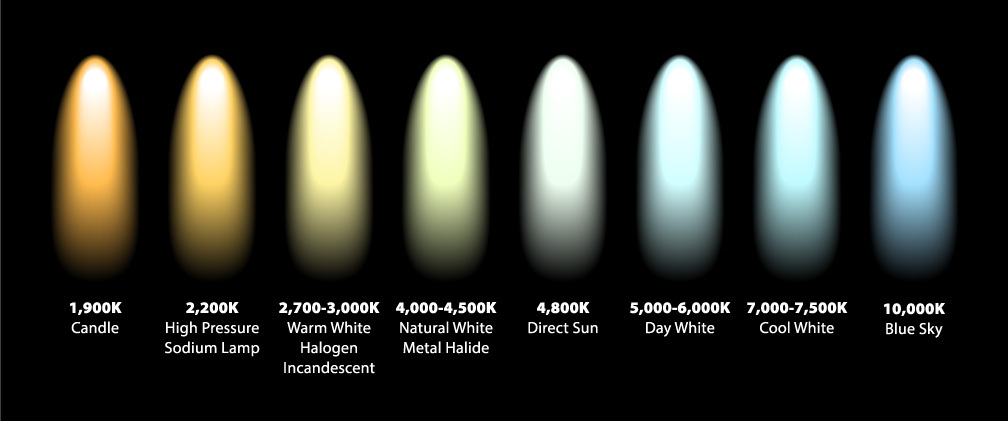
\includegraphics[width=0.9\linewidth]{Pictures/couleur_flammes.jpg}
    \caption{Couleur d'une flamme en fonction de sa température. Source : Inline Electric.}
    \label{fig:flammes_couleurs}
\end{figure}

\subsection*{Exemple : changement d'état}

Nous allons maintenant étudier une situation différente : nous ne travaillons plus dans une situation adiabatique mais isotherme, et le système échange de l'énergie avec l'environnement.

C'est le cas par exemple lors qu'un changement d'état, si l'on fait bouillir de l'eau dans une casserole. La réaction que l'on considère est la suivante :
\begin{equation}
    \ce{H2O(l) -> H2O(g)}
\end{equation}
La réaction est monobare et isotherme (elle se fait à la température de 100$^\circ$C), on a donc $\Delta H = Q$. Autrement dit, si on vaporise une quantité de matière $n$ d'eau, l'énergie thermique à fournir pour vaporiser l'eau est :
\begin{equation}
    Q = \Delta \mathcal{H} = \Delta_{vap} H^\circ \times n
\end{equation}
On se ramène en général à l'enthalpie massique de vaporisation, $L_{vap} = \Delta_{vap} H^\circ/M_{H_2O}$ de sorte que l'on puisse écrire l'énergie à fournir pour vaporiser une masse $m= M_{H_2O} n$ d'eau :
\begin{equation}
    Q = m L_{vap}
\end{equation}


\section{Loi de Hess}

Nous avons vu l'intérêt de connaître une enthalpie standard de réaction. Cependant, il serait laborieux de tabuler les enthalpies standard de toutes les réactions chimiques possibles. Pour simplifier le travail, il est utile de se ramener à des réactions chimiques de référence. Nous définissons pour cela l'état standard de référence d'un élément chimique\footnote{Rappel : un \textbf{élément} chimique est un élément du tableau périodique, à la différence d'un \textbf{constituant} qui peut être une molécule, un ion ou un solide cristallin.}:
\begin{definition}[\'{E}tat standard de référence d'un élément chimique]
    L’état standard de référence d’un élément chimique est le corps simple (c'est-à-dire le constituant chimique contenant uniquement cet élément) le plus stable à la pression $P\degree$. Il peut dépendre de la température $T$.
\end{definition}
\begin{example}
    A température ambiante, voici quelques états standard de référence :
    \begin{itemize}
        \item Oxygène \ce{O} : le dioxygène gazeux \ce{O2}
        \item Hydrogène \ce{H} : le dihydrogène gazeux \ce{H2}
        \item Carbone \ce{H} : le carbone graphite, un solide cristallin \ce{C}
    \end{itemize}
\end{example}

Une fois que l'on a défini les états standard de référence, on peut alors définir la réaction standard de formation d'une espèce chimique, dont nous pourrons tabuler l'enthalpie standard :
\begin{definition}[Réaction et enthalpie standard de formation]
    La réaction standard de formation d’un composé est la réaction de formation de ce composé, avec un coefficient stœchiométrique 1, à partir de ses éléments chimiques pris dans leur état standard de référence. L’enthalpie standard de cette réaction est l’enthalpie standard de formation du composé, notée $\Delta_f H\degree(T)$.
\end{definition}
\begin{remark}
    Attention, l'enthalpie de formation est toujours définie avec un coefficient stoechiométrique de 1 pour le corps étudié. Cela amène parfois à avoir des coefficients stoechiométriques non entiers ailleurs dans l'équation chimique.
\end{remark}
\begin{example}
    L'enthalpie standard de formation de l'eau \ce{H2O} correspond à l'enthalpie standard de réaction de formation de l'eau à la température $T$. L'état standard de référence des éléments chimiques constitutifs de l'eau est le dioxygène et le dihydrogène. La réaction standard de formation de l'eau à température ambiante s'écrit ainsi :
    \begin{equation}
        \ce{\frac{1}{2}O2(g) + H2(g) -> H2O(l)}
    \end{equation}
    et l'enthalpie standard de formation de l'eau est l'enthalpie de cette réaction.
\end{example}

Les chimistes ont mesuré par l'expérience les enthalpies standard de formation de la plupart des composés chimiques usuels. Cela permet de calculer l'enthalpie standard de n'importe quelle réaction chimique, par la loi de Hess :
\begin{theorem}[Loi de Hess]
    On considère une réaction chimique faisant intervenir des composés chimiques $A_i$ avec les coefficients stœchiométriques algébriques $\nu_i$. On prend pour convention $\nu_i <0$ pour les réactifs et $\nu_i>0$ pour les produits. Si on note $\Delta_fH\degree(A_i)$ l'enthalpie standard de formation du composé $A_i$, alors l'enthalpie standard de la réaction s'écrit :
    \begin{equation}
        \Delta_r H \degree = \sum_i \nu_i \Delta_f H\degree(A_i)
    \end{equation}
\end{theorem}
\begin{demonstration}
    Pour prouver cette loi, nous considérons une réaction en deux étapes :
    \begin{itemize}
        \item Dans une première étape, les éléments constitutifs des réactifs dans leur état standard sont séparés et mis dans leur état standard de référence ;
        \item Dans une seconde étape, ces éléments constitutifs sont rassemblés pour former les produits de la réaction chimique dans leur état standard.
    \end{itemize}

    Comme l'enthalpie est une variable d'état, elle ne dépend pas du chemin suivi. L'enthalpie standard de réaction est donc la somme des enthalpies standard de ces deux réactions :
    \begin{itemize}
        \item La deuxième réaction est la plus simple : elle correspond à la réaction standard de formation des produits avec leurs coefficients stoechiométriques respectifs. Son enthalpie standard est donnée par :
        \begin{equation}
            \Delta_r H\degree_2 = \sum_{\mathrm{produits}\,A_i} \nu_i \Delta_f H\degree(A_i)
        \end{equation}
        \item La première réaction est l'opposé de la réaction standard de formation des réactifs avec leurs coefficients stoechiométriques respectifs. Son enthalpie standard est donnée par :
        \begin{equation}
            \Delta_r H\degree_1 = - \sum_{\mathrm{reactifs}\,A_i} |\nu_i|\Delta_f H\degree(A_i)
        \end{equation}
    \end{itemize}
    On en déduit bien l'expression obtenue pour la loi de Hess.
\end{demonstration}
\begin{example}
    La démonstration est un peu abstraite. Pour qu'elle soit plus claire, nous pouvons prendre l'exemple de la réaction de combustion du propane que nous avons déjà étudiée plus haut :
    \begin{equation}
    \ce{C3H8 (g) + 5 O2 (g) -> 3 CO2 (g) + 4 H2O (g)}
\end{equation}
Dans leur état standard, tous les composés chimiques de cette réaction sont gazeux. La première réaction consiste à séparer les éléments chimiques dans leur état standard de référence :
\begin{equation}
    \ce{C3H8(g) + 5O2(g) -> 3 C(s) + 4 H2(g) + 5 O2(g) }
\end{equation}
Les 5 molécules de dioxygène se simplifient de part et d'autre et on obtient l'inverse de la réaction standard de formation du propane, dont l'enthalpie standard de réaction est :
\begin{equation}
    \Delta_r H\degree_1 = - \Delta_f H\degree(\ce{C3H8 (g)})
\end{equation}
La seconde réaction consiste à former les produits à partir des éléments chimiques :
\begin{equation}
    \ce{3 C(s) + 4 H2(g) + 5 O2(g) -> 3 CO2(g) + 4 H2O(l) }
\end{equation}
Il s'agit de la réaction standard de formation de 4 molécules d'eau et 3 molécules de dioxyde de carbone. Celle-ci a une enthalpie de réaction :
\begin{equation}
    \Delta_r H\degree_2 = 3\Delta_f H\degree(\ce{CO2 (g)}) + 4\Delta_f H\degree(\ce{H2O (g)})
\end{equation}
On en déduit l'enthalpie standard de la réaction :
\begin{equation}
    \Delta_r H\degree = - \Delta_f H\degree(\ce{C3H8 (g)}) + 3\Delta_f H\degree(\ce{CO2 (g)}) + 4\Delta_f H\degree(\ce{H2O (g)})
\end{equation}
On retrouve bien la loi de Hess, puisque le'enthalpie standard de formation du dioxygène gazeux est nulle (c'est déjà un corps simple dans son état standard de référence).
\end{example}

\begin{remark}
    Dans un concours, il est inutile de refaire cette démonstration : vous pouvez utiliser la loi de Hess directement. Cette démonstration est là pour que vous puissiez comprendre pourquoi cette loi est valable, et pourquoi il est utile de définir toutes ces variables standard. En général, on ne vous donnera jamais une enthalpie standard de réaction car celles-ci ne sont pas tabulées. Il faudra la calculer à partir de la loi de Hess.
\end{remark}



\end{document}